\documentclass[review]{elsarticle}
\usepackage{lineno,hyperref}
\modulolinenumbers[5]
\usepackage[margin=1in]{geometry}
\usepackage{graphicx}
\usepackage{placeins}
\usepackage{comment}
\usepackage{color}

\journal{Journal of Nuclear Materials}
\bibliographystyle{elsarticle-num}

\begin{document}
\begin{frontmatter}
\title{Molecular dynamics investigations of interface effects in Fe-Ni-Al}

\author[davisa,berka]{Benjamin Beeler\corref{qwe}}
\cortext[qwe]{Corresponding author}
\ead{bwbeeler@ucdavis.edu}
\author[berka]{Mark Asta}
\author[berkb]{Peter Hosemann}
\author[davisa,davisb]{Niels Gr$\o$nbech-Jensen}
\address[davisa]{Department of Mechanical and Aerospace Engineering, University of California, Davis, CA 95616}
\address[berka]{Department of Materials Science, University of California, Berkeley, CA 94720}
\address[berkb]{Department of Nuclear Engineering, University of California, Berkeley, CA 94720}
\address[davisb]{Department of Mathematics, University of California, Davis, CA 95616}

\begin{abstract}
Under heat treatment, maraging steels form coherent NiAl precipitates that can significantly increase the macroscopic strength of the material.  The precipitates formed in these materials may act as sinks for defects, similar to oxide-dispersion strengthened steels (ODS).  This work presents computational investigations aimed at better understanding the role of coherent precipitates in increasing radiation tolerance in maraging steels.  Interatomic potentials have been developed for the description of Fe-Ni-Al alloys, to simulate an ideal alloy of BCC Fe with NiAl precipitates, and associated Fe/NiAl planar interfaces.  Characteristics and energetics of the interfaces are analyzed, the interaction of point defects with planar and spherical interfaces is studied, and finally, radiation cascades are induced in proximity to the interfaces, whereafter the effect of the interface on defect accumulation is investigated.
\end{abstract}
\end{frontmatter}

\linenumbers

\section{Introduction}

Structural materials for nuclear applications suffer a wide range of property changes as a consequence of swelling, changes in the dislocation structures, solute segregation, and radiation-enhanced and -induced precipitation \cite{odette2008,olander,stiegler1979,was2007}.  The consequences of these effects include hardening, embrittlement, low-temperature irradiation creep, void swelling, and loss of ductility and creep resistance.  The formation of cascades due to particle irradiation and the formation of a large number of point defects cannot be avoided initially.  However, recent studies have shown that the formation of large defects can be delayed or avoided by trapping the defects at a large number of defect sinks (namely, interfaces such as grain boundaries) where the defects annihilate, preventing their accumulation within the lattice.  

For these reasons, nanostructured ferritic alloys (NFAs), such as oxide-dispersion strengthened (ODS) alloys, are considered as candidate materials for nuclear applications.  Recent research on ODS alloys and multilayer materials has shown that providing sufficient interfaces in a material can increase the material's radiation tolerance and reduce helium embrittlement.  However, ODS alloys have the disadvantage that materials processing is very difficult and expensive.  

It has been shown that heat treatments on maraging steels lead to the formation of finely dispersed intermetallic Ni-Al based precipitates \cite{decker1988,stiller2008,schnitzer2010}.  Benefits of these materials are that they are much cheaper to manufacture and process than ODS steels and that these steels are widely used and available in industry, allowing one to benefit from already published data on the alloys.  

Thus, it is of interest to determine if intermetallic coherent precipitates in maraging steels can be used in a similar way to oxide precipitates in ODS steels, i.e., to remove radiation damage from the matrix and increase the radiation tolerance of the material.  

Molecular dynamics (MD) has been shown to be an effective tool for the investigation of material properties on an atomistic scale.  Utilizing empirical or semi-empirical descriptions of atomic interactions, MD is a methodology that provides reasonable computational expense, generality and accuracy.  It is the aim of this research to utilize MD simulations to investigate the fundamental behavior of the Fe-Ni-Al system on an atomistic scale.  This will allow for the investigation of the effect of coherent NiAl precipitates on the radiation tolerance of maraging steels.

In this paper, interatomic potentials are developed for the description of Fe-Ni-Al alloys, to simulate an ideal alloy of BCC Fe with NiAl precipitates, and associated Fe/NiAl planar interfaces.  Characteristics and energetics of the interfaces are analyzed, the interaction of point defects with planar and spherical interfaces is studied, and finally, radiation cascades are induced in proximity to the interfaces, whereafter the effect of the interface on defect accumulation is investigated.


\section{Potential Fitting}
Potential functions in the EAM \cite{daw1984} formalism are taken from the literature for the pure Fe system \cite{mendelev2003}, as well as for the Ni-Al binary system \cite{pun2009}.  Thus, the task is to fit Fe-Al and Fe-Ni interactions to generate a ternary Fe-Ni-Al interatomic potential.  

The LAMMPS \cite{plimpton1995} software package is utilized for molecular statics and dynamics simulations involving these binary and ternary systems.  Potentials are thus written in the setfl format.  Before fitting procedures can begin, it is required to adjust the limits on the ranges of electron density and cutoff distance such that consistent values exist for the Fe system and the Ni-Al system.  The \textit{drho} (electron density step) and the \textit{dr} (distance step) from the Ni-Al interatomic potential are taken as the standard for our ternary potentials.  In this case, only the Fe potential has a need to undergo scaling to a new drho and dr value.  Interpolation is then performed using a 5-point Langrangian polynomial fit.  

The first step in the fitting procedure involves an invariant scaling.  The quantity $\bar{\rho}$  is given by the sum:

\begin{equation}
\bar{\rho} = \sum_{j \neq i} \rho(r_{ij})
\end{equation}

where $\rho$ is the electron density.  The energy and forces in the system are invariant to the scaling of the electron density and the embedding energy,

\begin{equation}
\rho(r_{ij}) = \alpha\rho(r_{ij})
\end{equation}

\begin{equation}
F(\bar{\rho}) = F(\frac{\bar{\rho}}{\alpha}) 
\end{equation}

where \textit{F} is the embedding energy and $\alpha$ is a scale factor.  This scaling does not change the properties of the pure systems, but does in fact change the behavior of the alloy.  In our work, only the Fe electron density and embedding energy have been scaled.  Given a value of $\alpha$, only the pair potentials for the Fe-Al and Fe-Ni systems are left to be characterized.  

The pair potentials for Fe-Al and Fe-Ni interactions are described by a pairwise function in the form of:

\begin{equation}
\phi = \left\{ \begin{array}{lcr}
		\frac{Z^{2}q_{e}^{2}}{r}\psi(\frac{r}{r_{s}}) & for & r < r_{1} \\
		p(t) & for & r_{1} < r < r_{2} \\
		\sum\limits_{k=1}^{n^{\phi}} a_{k}^{\phi}(r_{k}^{\phi}-r)^{3}\theta(r_{k}^{\phi}-r) & for & r > r_{2} \\
		\end{array} \right.\ 
\end{equation}

where Z is the atomic number, q$_{e}$ is the charge on an electron, 

\begin{equation}
r_{s} = 0.88534\frac{r_{B}}{2^{1/2}Z^{1/3}}
\end{equation}

where r$_{B}$ is the Bohr radius,

\begin{equation}
\psi(x) = 0.1818exp^{-3.2x} + 0.5099exp^{-0.9423x} + 0.2802exp^{-0.4029x} + 0.02817exp^{-0.2016x}
\end{equation}

p(t) is the cubic hermite spline function,

\begin{equation}
	p(t) = h_{00}(t)p_{0} + h_{10}(t)m_{0} + h_{01}(t)p_{1} + h_{11}(t)m_{1}
\end{equation}

where m$_{0}$ and p$_{0}$ are the slope and evaluation, respectively, of $\phi$(r) at r$_{1}$, m$_{1}$ and p$_{1}$ are the slope and evaluation, respectively of $\phi$(r) at r$_{2}$, and h$_{ij}$ is given below.

\begin{equation}
h_{00}(t) = 2t^{3} - 3t^{2} + 1
\end{equation}

\begin{equation}
h_{10}(t) = t^{3} - 2t^{2} + 1
\end{equation}

\begin{equation}
h_{01}(t) = -2t^{3} + 3t^{2} 
\end{equation}

\begin{equation}
h_{11}(t) = t^{3} - t^{2}
\end{equation}

\begin{equation}
t = \frac{r - r_{1}}{r_{2} - r_{1}}
\end{equation}

and $\theta(x)$ is the Heaviside step function.

The total number of knots in the cubic spline is set to seven, thus n$^{\phi}$ is set to seven in equation 4 and the total number of fitting coefficients (a$_{k}^{\phi}$ in equation 4) is also seven.

Seven targets were utilized in the fitting of each potential:  formation energy and lattice parameter of B2-FeX, L1$_{2}$-Fe$_{3}$X and D0$_{3}$-Fe$_{3}$X, as well as the formation energy of B2-FeX under pressure (X=Ni/Al).  Each fitting target was assigned a weight.  Pair potential functions were initialized with null coefficients and the fitting parameter $\alpha$ was manually varied to approach a local minimum.  The value of $\alpha$ was thus set at 0.00175.  The iterative process varied all seven coefficients simultaneously, utilizing seven unique associated random steps.  The maximum allowable step was $\pm$ 0.05.  If a given set of random steps produced a reduction in the overall error (defined as the summation of the absolute value of each target parameter error multiplied by the respective target parameter weight), the step is accepted and the coefficients are updated.  This fitting procedure is repeated until the error reaches a sufficiently low level.  This fitting procedure proved quite successful in generating a number of potentials that can adequately produce appropriate results for the fitting targets.  

After an initial fitting procedure yielded suitable cross potentials for the Fe-Ni and Fe-Al systems, testing began to evaluate the effectiveness of the potential at predicting a variety of properties not included into the fitting.  The potential performed quite well at predicting formation energies and lattice constants of intermetallic structures not included in the fitting targets.  However, this system of testing revealed that the ternary potential was yielding negative interfacial energies.  It was found that the potential was predicting an unrealistic low-energy ordered structure consisting of consecutive layers of Fe-Ni-Al residing on a BCC super lattice.  Utilizing this information, a final target parameter was implemented into the fitting of the ternary potential.  The formation energy of the BCC-based layered Fe-Ni-Al was determined utilizing density functional theory calculations.  Implementation of this final fitting parameter allowed for an additional stage of potential tuning and ensured that a wider range of applicability exists for this potential, including interfacial systems.  

The parameters describing the resultant potential are given in Table 1. 

\textcolor{red}{I remade these potentials. Refitted and made sure that ZBL was splined onto them. Splining via lammps. I am still not happy with the shape of the FeNi pair potential. Some of the structures are linesearch alpha 0 or max force iterations, so maybe metastable. Should I look at elastic constants to test? Should I do thermal expansion studies?}

\begin{table}[htbp]
\caption{The parameters describing the FeAl and FeNi cross potentials.  All distances are expressed in \AA{}.}
\begin{center}
\begin{tabular}{|c|c|c|}
	\hline
	& FeAl & FeNi  \\
	 \hline
	 r$_{1}$ & 1.0 & 1.2  \\
	 r$_{2}$ & 2.0 & 2.0 \\
	 a$_{1}^{\phi}(r_{1}^{\phi}$) & 0.935399151361639(2.5) & -0.0930063002589449(2.5)  \\
	 a$_{2}^{\phi}(r_{2}^{\phi}$) & 2.12706494073913(3.0) & 0.0950516635353975(3.0) \\
	 a$_{3}^{\phi}(r_{3}^{\phi}$) & -1.58853173072582(3.5) & 0.0960585680950139(3.5)  \\
	 a$_{4}^{\phi}(r_{4}^{\phi}$) & 0.942835290353412(4.0) & 0.0203771265673911(4.0)  \\
	 a$_{5}^{\phi}(r_{5}^{\phi}$) & -0.311367683104878(4.5) & 0.201314655488025(4.5)  \\
	 a$_{6}^{\phi}(r_{6}^{\phi}$) & 0.151610678422719(5.0) & -0.0854904597821776(5.0)  \\
	 a$_{7}^{\phi}(r_{7}^{\phi}$) & -0.0584089034579909(5.5) & -0.0277597349060834(5.5)  \\
	  \hline
\end{tabular}
\end{center}
\label{default}
\end{table}%

The physical properties calculated using the Fe-Ni-Al EAM potential, associated fitting targets from VASP, and fitting weights are tabulated in table 2.  If not explicitly referenced, VASP calculations were performed as a part of this work.

\begin{table}[htbp]
\caption{The target parameter physical properties calculated with the Fe-Ni-Al ternary interatomic potential and associated weights.  Energies given in eV and distances given in \AA{}.}
\begin{center}
\begin{tabular}{|c|c|c|c|}
	\hline
	& This Work & VASP & Weights \\
	 \hline
	 B2-FeNi E$_{f}$/\textit{at} & 0.084 & 0.084 & 0.3 \\
	 B2-FeNi a$_{0}$ & 2.841 & 2.854 & 0.3 \\
	 L1$_{2}$-Fe$_{3}$Ni E$_{f}$/\textit{at} & 0.139 & 0.048 & 0.08 \\
	 L1$_{2}$-Fe$_{3}$Ni a$_{0}$ & 3.673 & 3.578 & 0.08 \\
	 D0$_{3}$-Fe$_{3}$Ni E$_{f}$/\textit{at} & 0.032 & 0.034 & 0.08 \\
	 D0$_{3}$-Fe$_{3}$Ni a$_{0}$ & 5.762 & 5.718 & 0.08  \\
	 B2-FeNi E$_{f}$/\textit{at} a$_{0}$=2.7& 0.286 & 0.287 & 0.08 \\
	 B2-FeAl E$_{f}$/\textit{at} & -0.333 & -0.334 & 0.3  \\
	 B2-FeAl a$_{0}$ & 2.878 & 2.875 & 0.3 \\
	 L1$_{2}$-Fe$_{3}$Al E$_{f}$/\textit{at} & -0.137 & -0.117 & 0.08 \\
	 L1$_{2}$-Fe$_{3}$Al a$_{0}$ & 3.5848 & 3.797 & 0.08 \\
	 D0$_{3}$-Fe$_{3}$Al E$_{f}$/\textit{at} & -0.244 & -0.201 & 0.08 \\
	 D0$_{3}$-Fe$_{3}$Al a$_{0}$ & 5.688 & 5.986 & 0.08  \\
	 B2-FeAl E$_{f}$/at a$_{0}$=2.4 & 2.564 & 2.558 & 0.08  \\
	 Layered BCC-FeNiAl E$_{f}$/\textit{at}& 0.052 & 0.149 & 0.09 \\
	 \hline
\end{tabular}
\end{center}
\label{default}
\end{table}%

The potential was then applied to non-targeted systems.  In table 3 and table 4, for the Fe-Ni and Fe-Al systems, respectively, the formation energies and lattice constants for the B2, L12 and D03 intermetallic structures calculated with the Fe-Ni-Al EAM potential are compared against DFT values and other interatomic potentials.    

\begin{table}[htbp]
\caption{The formation energy and lattice constant of the B2, L12 and D03 Fe-Ni intermetallic compounds.  The results for this work, first principles calculations, and other Fe-Ni potential formulations are presented for comparison.}
\begin{center}
\begin{tabular}{|c|c|c|c|c|}
	\hline
	& This Work & VASP\cite{mishin2005} & Bonny \cite{bonny2009} & Mishin\cite{mishin2005} \\
	 \hline
	 L1$_{2}$-FeNi$_{3}$ E$_{f}$/\textit{at} & 0.038 & -0.089 & -0.073 & ~-0.09 \\
	 L1$_{2}$-FeNi$_{3}$ a$_{0}$ & 3.521 & 3.545 & - & 3.563 \\
	 D0$_{3}$-FeNi$_{3}$ E$_{f}$/\textit{at} & 0.023 & 0.024 & - & ~-0.01 \\
	 D0$_{3}$-FeNi$_{3}$ a$_{0}$ & 5.586 & 5.643 & - & - \\
	 
	 	 \hline
\end{tabular}
\end{center}
\label{default}
\end{table}%

\begin{table}[htbp]
\caption{The formation energy and lattice constant of the B2, L12 and D03 Fe-Al intermetallic compounds.  The results for this work, first principles calculations, and other Fe-Al potential formulations are presented for comparison.}
\begin{center}
\begin{tabular}{|c|c|c|c|}
	\hline
	& This Work & VASP & Mendelev\cite{mendelev2005} \\
	 \hline
	 L1$_{2}$-FeAl$_{3}$ E$_{f}$/\textit{at} & -0.110 & -0.117  & -0.103 \\
	 L1$_{2}$-FeAl$_{3}$ a$_{0}$ & 3.899 & 3.797 & 3.786  \\
	 D0$_{3}$-FeAl$_{3}$ E$_{f}$/\textit{at} & -0.120 & -0.024 & -0.004 \\
	 D0$_{3}$-FeAl$_{3}$ a$_{0}$ & 6.131 & 5.986 & 5.969 \\	 
	 	 \hline
\end{tabular}
\end{center}
\label{default}
\end{table}%

It should be noted that this potential performs less effectively, albeit still adequately, for Ni-rich or Al-rich structures than for Fe-rich structures.  

%The focus of this potential was to describe the Fe-Ni-Al system for maraging allows.  Hence, the primary systems of interest are

\section{Computational Details}
Molecular dynamics and statics simulations are performed utilizing the LAMMPS \cite{plimpton1995} software package.  We utilize the GJF thermostat \cite{gjf2013, gjf2014} (fix langevin gjf) due to its robust configurational sampling properties.  The damping parameter (analogous to relaxation time) is set to 1 ps.  Further simulation details are provided within each section.

\section{Results}
\subsection{Fe-Ni-Al Interfacial Energies}
A supercell is constructed of BCC-Fe and B2-NiAl such that an equal amount of each structure is present within the supercell, and that two coherent interfaces exist (see Figure 1).  Systems of varying length normal to the interface and of varying interfacial area are investigated to ensure that interfaces are not interacting with one another, and that the interfacial energy pure area is independent of the size of the interface or the length of the supercell.  Three interfacial orientations were investigated: (100), (110) and (111).  Each of these systems was equilibrated at 100 K for 100 ps, with averaging performed over the final 50 ps of the simulation.  The equilibration was performed in a constrained NPT ensemble, with the direction normal to the interface allowed to relax and the in-plane directions of the interface fixed.  The fixed lattice constant was set to the average of the BCC-Fe and B2-NiAl lattice constants at 100 K to minimize strain.  

The results for interfacial energies at 100 K for each of the three orientations is presented in Table 5.


\begin{figure}[hp]
   \centering
   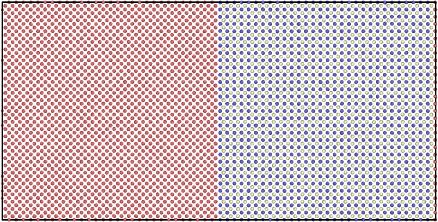
\includegraphics[width=\textwidth]{figure_nf.png} 
   \caption{System of BCC-Fe and B2-NiAl with two (100) planar interfaces.  One interface resides in the center of the supercell, the other interface resides at either end of the supercell, due to periodic boundaries.  Red atoms are Fe; Blue atoms are Ni; Yellow atoms are Al.}
   \label{fig:example}
\end{figure}

\begin{table}[htbp]
\caption{Interfacial energies for the BCC-Fe/B2-NiAl (100), (110) and (111) planar interfaces at 100 K.}
\begin{center}
\begin{tabular}{|c|c|}
	\hline
	& Interfacial Energy (J/cm$^{2}$)  \\
	 \hline
	 (100) & 0.218  \\
	 (110) & 0.064  \\
	 (111) & 0.084  \\
	  	 \hline
\end{tabular}
\end{center}
\label{default}
\end{table}%

It is seen that the (110) planar interface has the lowest interfacial energy.  This makes qualitative sense, as the (110) plane is the close-packed plane in the BCC crystal structure.  It should also be noted the magnitude of the interfacial energies.  The interfacial energy for all three orientations is very low.  Since these are coherent interfaces, this is expected.  

\subsection{Interaction of Point Defects with Interfaces}
includes planar and spherical
\subsubsection{Planar Interfaces}
A two-phase setup identical to that described in section 4.1 is utilized for the investigation of point defect properties near planar interfaces.  A single point defect (vacancy or interstitial) is inserted in close proximity to the planar interface.  The formation energy of the defect is determined from

\begin{equation}
E_{f}^{def} = E_{f-sys}^{def} - N*E_{f-sys}^{nf}/atom
\end{equation}

where E$_{f}^{def}$ is the formation energy of the system with a defect, E$_{f}^{nf}/atom$ is the formation energy per atom of the system without a defect (nf = interface), and \textit{N} is the number of atoms in a system with a defect.  The formation energy of the system with an interface is determined from

\begin{equation}
E_{f-sys}^{nf} = E_{sys}^{nf} -  N^{Fe}*E^{Fe}/atom - N^{B2}*E^{B2}/atom
\end{equation}

where E$_{sys}^{nf}$ is the total energy of the system with an interface, N$^{Fe}$ is the number of Fe atoms in the system,  E$^{Fe}/atom$ is the equilibrium energy per atom of BCC Fe, N$^{B2}$ is the number of B2-NiAl atoms in the system, and E$^{B2}/atom$ is the equilibrium energy per atom of B2-NiAl.  

The defect is progressively moved farther away from the interface, and the energy at each step is calculated in order to construct the formation energy of a point defect as a function of the depth from the interface.  This can provide information to the energetic attraction between these interfaces and point defects.  These simulations are performed at 0 K to eliminate any possible diffusion of defects, allowing the investigation of only the defect formation energy.

The results for a vacancy and an interstitial for all three planar interfacial orientations are displayed in Figure 2 and Figure 3, respectively.

\begin{figure}[htp]
   \centering
   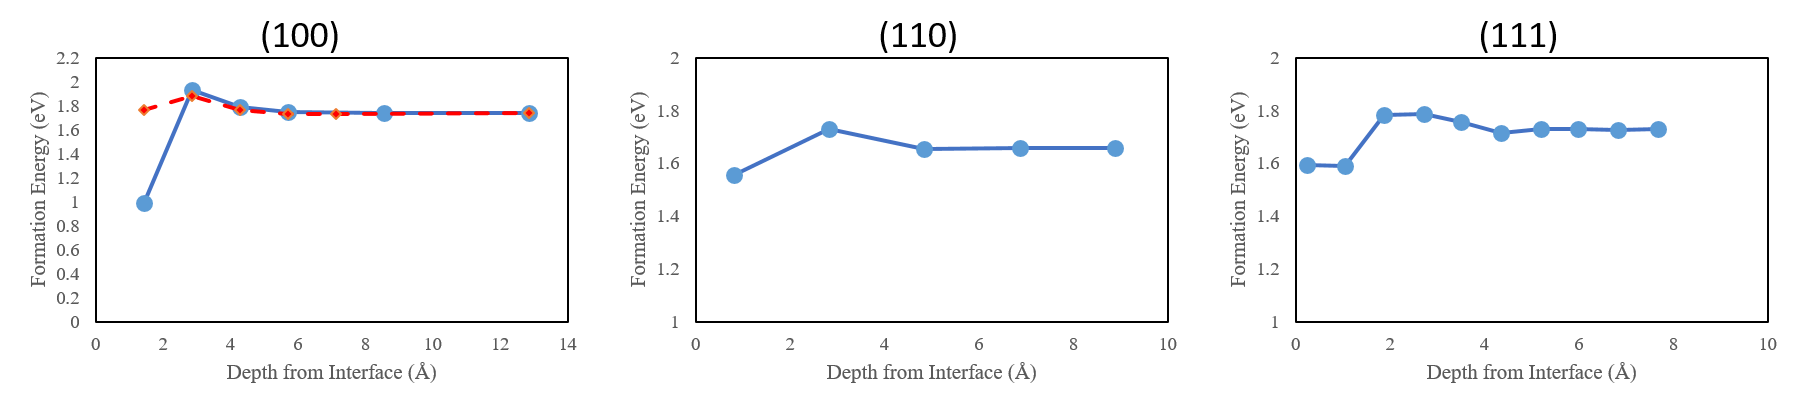
\includegraphics[width=\textwidth]{vac_nf.png} 
   \caption{The formation energy of a vacancy as a function of depth from a planar interface at 0 K.  Results are shown for three interfacial orientations.  Formation energies are given in eV and depth is given in Angstroms.  For the (100) interface, the blue points and solid line denote an interface where the B2-NiAl terminal is a plane of Ni atoms.  The red points and dashed line denote an interface where the B2-NiAl terminal is a plane of Al atoms.  No such terminal differences exist in the (110) and (111) cases.}
   \label{fig:example}
\end{figure}

\begin{figure}[htp]
   \centering
   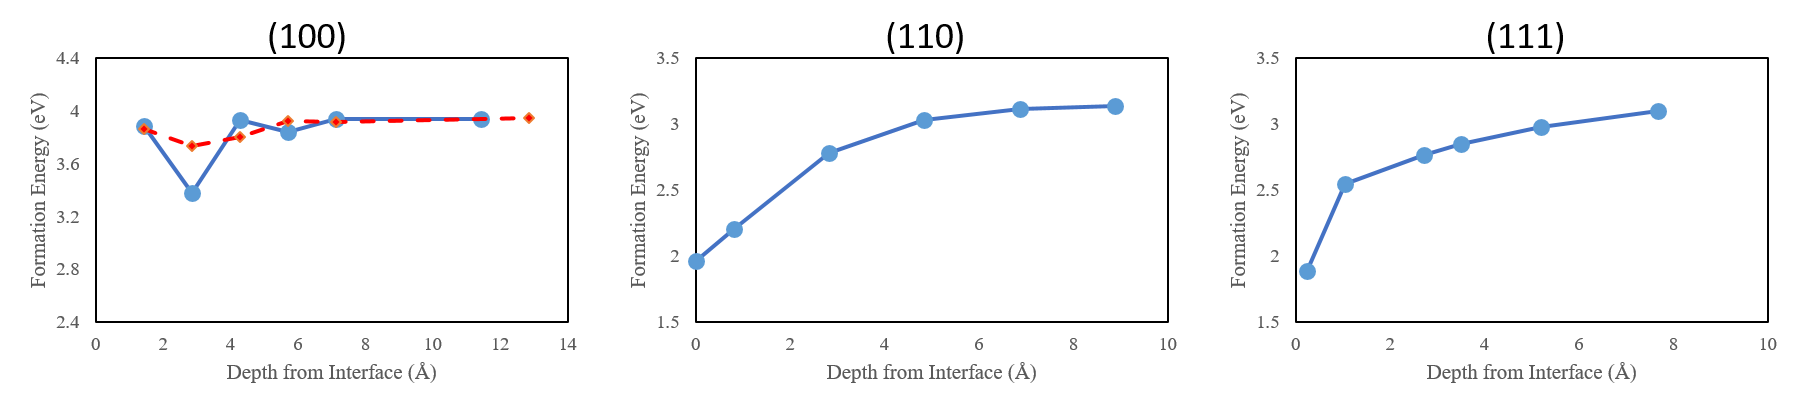
\includegraphics[width=\textwidth]{int_nf.png} 
   \caption{The formation energy of an interstitial as a function of depth from a planar interface at 0 K.  Results are shown for three interfacial orientations.  Formation energies are given in eV and depth is given in Angstroms.  For the (100) interface, the blue points and solid line denote an interface where the B2-NiAl terminal is a plane of Ni atoms.  The red points and dashed line denote an interface where the B2-NiAl terminal is a plane of Al atoms.  No such terminal differences exist in the (110) and (111) cases.}
   \label{fig:example}
\end{figure}

The first information interpreted from these figures is that the energetic interaction is relatively short ranged.  Once a defect is more than 2-3 lattice spacings away from the interface, the defect is behaving, energetically, as if it is residing in the bulk.  For vacancies, the energetic interaction is typically relatively small, approximately 0.1 eV.  The one exception is for a vacancy near a Ni terminal in the (100) interfacial orientation, where a much stronger attraction is occurring.  For interstitials, the energetic interaction is typically much stronger than that of vacancies, at approximately 1 eV for the cases of the (110) and the (111) orientations.  For the (100) interface, the interaction is somewhat smaller.  
\FloatBarrier

\subsubsection{Spherical Precipitates}
To generate a spherical precipitate, a supercell of BCC-Fe is generated, a sphere of a given radius is created in the center of the supercell, Fe atoms within that sphere are replaced with the B2-NiAl lattice.  An example of this configuration is shown in Figure 4.  As in section 4.2.1, a defect is introduced near the spherical precipitate and the formation energy is calculated.  The defect is moved progressively farther from the interface to construct the formation energy of a point defect as a function of the depth from the interface.

\begin{figure}[htp]
   \centering
   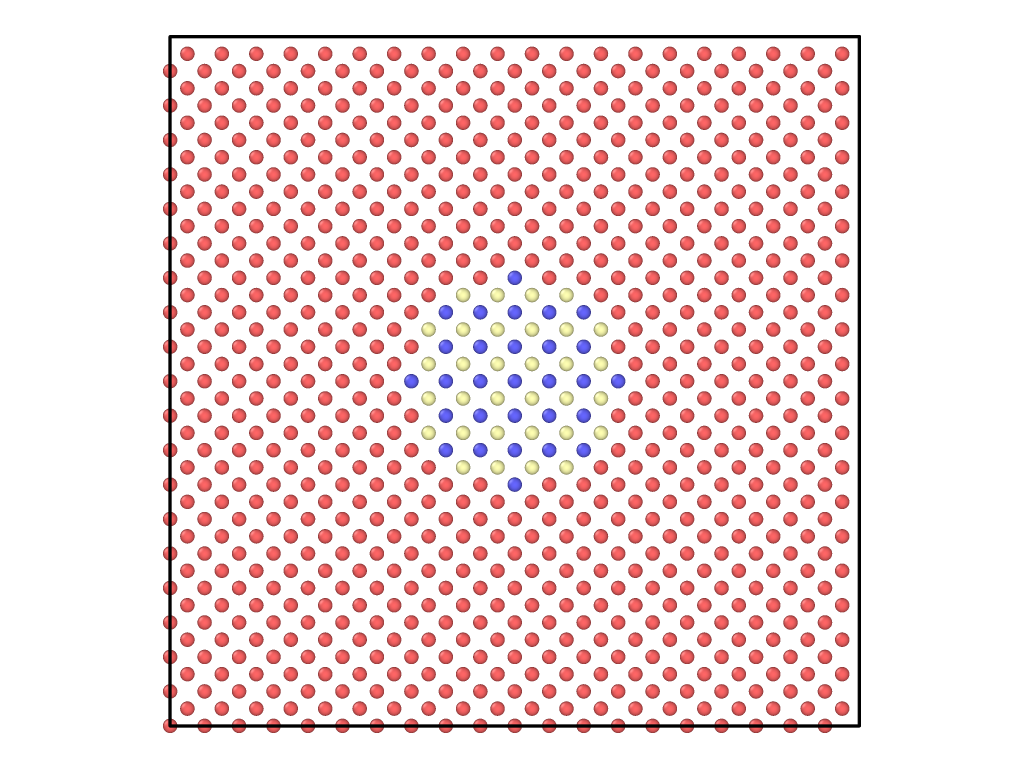
\includegraphics[width=\textwidth]{sphere_precip.png} 
   \caption{System of BCC-Fe with spherical B2-NiAl precipitate in center of supercell.  Image is a 2-D slice through a 3-D supercell.  Red atoms are Fe; Blue atoms are Ni; Yellow atoms are Al.}
   \label{fig:example}
\end{figure}

The results for a single vacancy and di-vacancy at 100 K are displayed in Figure 5 and Figure 6, respectively.  

\begin{figure}[htp]
   \centering
   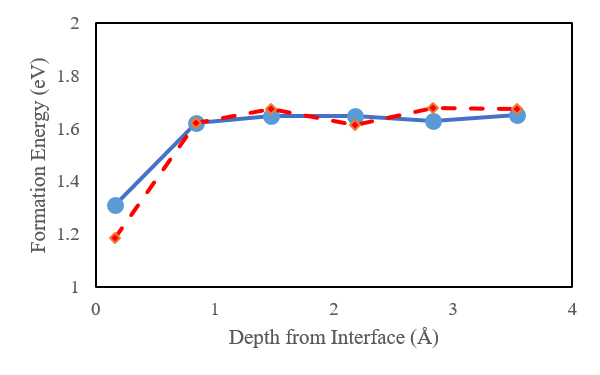
\includegraphics[width=0.5\textwidth]{vac_sphere.png} 
   \caption{System of BCC-Fe with spherical B2-NiAl precipitate in center of supercell.  Image is a 2-D slice through a 3-D supercell.  Red atoms are Fe; Blue atoms are Ni; Yellow atoms are Al.}
   \label{fig:example}
\end{figure}

\begin{figure}[htp]
   \centering
   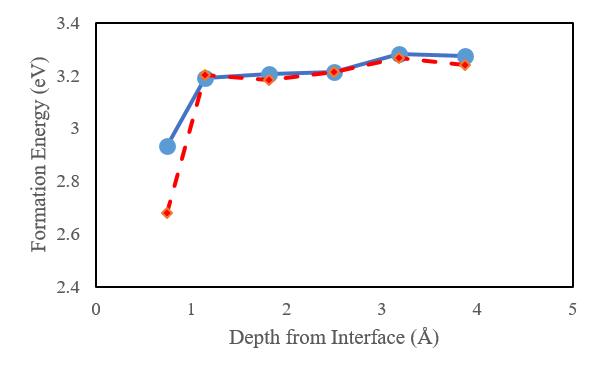
\includegraphics[width=0.5\textwidth]{divac_sphere.png} 
   \caption{System of BCC-Fe with spherical B2-NiAl precipitate in center of supercell.  Image is a 2-D slice through a 3-D supercell.  Red atoms are Fe; Blue atoms are Ni; Yellow atoms are Al.}
   \label{fig:example}
\end{figure}

It is seen from a comparison of Figure 5 to Figure 2, that very similar behavior is observed for planar interfaces and spherical precipitates.  The range of interaction between a vacancy and a spherical precipitate is only a few Angstroms.  When the vacancy is more than two lattice spacings away from the precipitate, it behaves energetically as if it resided in the bulk.  The magnitude of the close range interaction is also similar, in that it is on the order of a few tenths of an eV.  Thus, vacancies display an energetic attraction to spherical precipitates, but this attraction is fairly weak, and it is very short range.

For divacancies in Figure 6, it is observed that a similar range of interaction exists between the defect and the precipitate, when compared to monovacancies.  However, the magnitude of the short range energetic interaction is stronger, up to approximately 0.6 eV.  Thus, divacancies display an energetic attraction to spherical precipitates, this attraction is very short range, but is stronger than that of monovacancies.

Need to put some interstitials in for spheres... Maybe need to do some 0 K sphere work... Dont think I did this.

\FloatBarrier

\subsection{Defect Evolution Near Interfaces}
\subsubsection{Planar Interfaces}
With the information of how point defects energetically interaction with planar interfaces at 0 K, it is of interest to explore defect behavior at high temperature.  At high temperature, defects will be able to diffuse and cluster, and determining how these systems behave is not always clear from static energetic calculations.  

A two-phase configuration similar to that described in section 4.1 is utilized for the investigation of high temperature point defect behavior near planar interfaces.  A temperature of 600 K was chosen as this is a reasonable temperature for structural materials in nuclear reactors.  It has the added benefit of allowing for fairly rapid diffusion of interstitials and minimal diffusion of vacancies.  The system was equilibrated at 600 K for 100 ps.  Next, 50 Fe interstitials and 50 Fe vacancies were randomly inserted into the BCC-Fe matrix.  The system was then allowed for evolve for 1 ns.  

If we track the vacancies in the system, expected behavior is observed.  Very minimal diffusion of vacancies occurs, and some of the interstitials diffuse to find vacancies and annihilation takes place.  However if we track the interstitials in the system, quite different behavior is observed.  A representative example illustration is displayed in Figure 7.  In Figure 7, a coordination number sorting has been performed, such that the only atoms shown have a coordination number of 15 or higher, thus, only interstitial atoms or atoms surrounding interstitials are shown (there exist some thermal fluctuations that cause atoms to appear).  Initially, interstitials diffuse and form clusters.  These clusters vary in size and orientation.  Many of these clusters diffuse rapidly, forming larger clusters.  However, some mono-interstitials and interstitial clusters diffuse into the interface.  As time progresses, interstitial clusters random walk diffuse throughout the supercell, until they eventually diffuse into the interface.  By the end of the simulation, all of the interstitials and interstitial clusters have diffused to the interfaces and are effectively pinned at these interfaces.  Thus, in this simulation that contains only low energy coherent interfaces, the interfaces are acting as sinks for defects, effectively removing radiation damage from the system.  The importance of this result cannot be overstressed.  It is observed that coherent intermetallic interfaces are acting to remove radiation damage from the bulk Fe system.

It is suggested that further removal of vacancy defects can take place on a much longer time scale via interstitial ejection, as has been modeled in copper \cite{bai2010}.  It should also be noted that occasionally an immobile interstitial cluster is formed, and is thus not removed from the bulk system.  However, the most common type of interstitial clusters observed are sessile <111> clusters, which diffuse quite rapidly.  

\begin{figure}[htp]
   \centering
   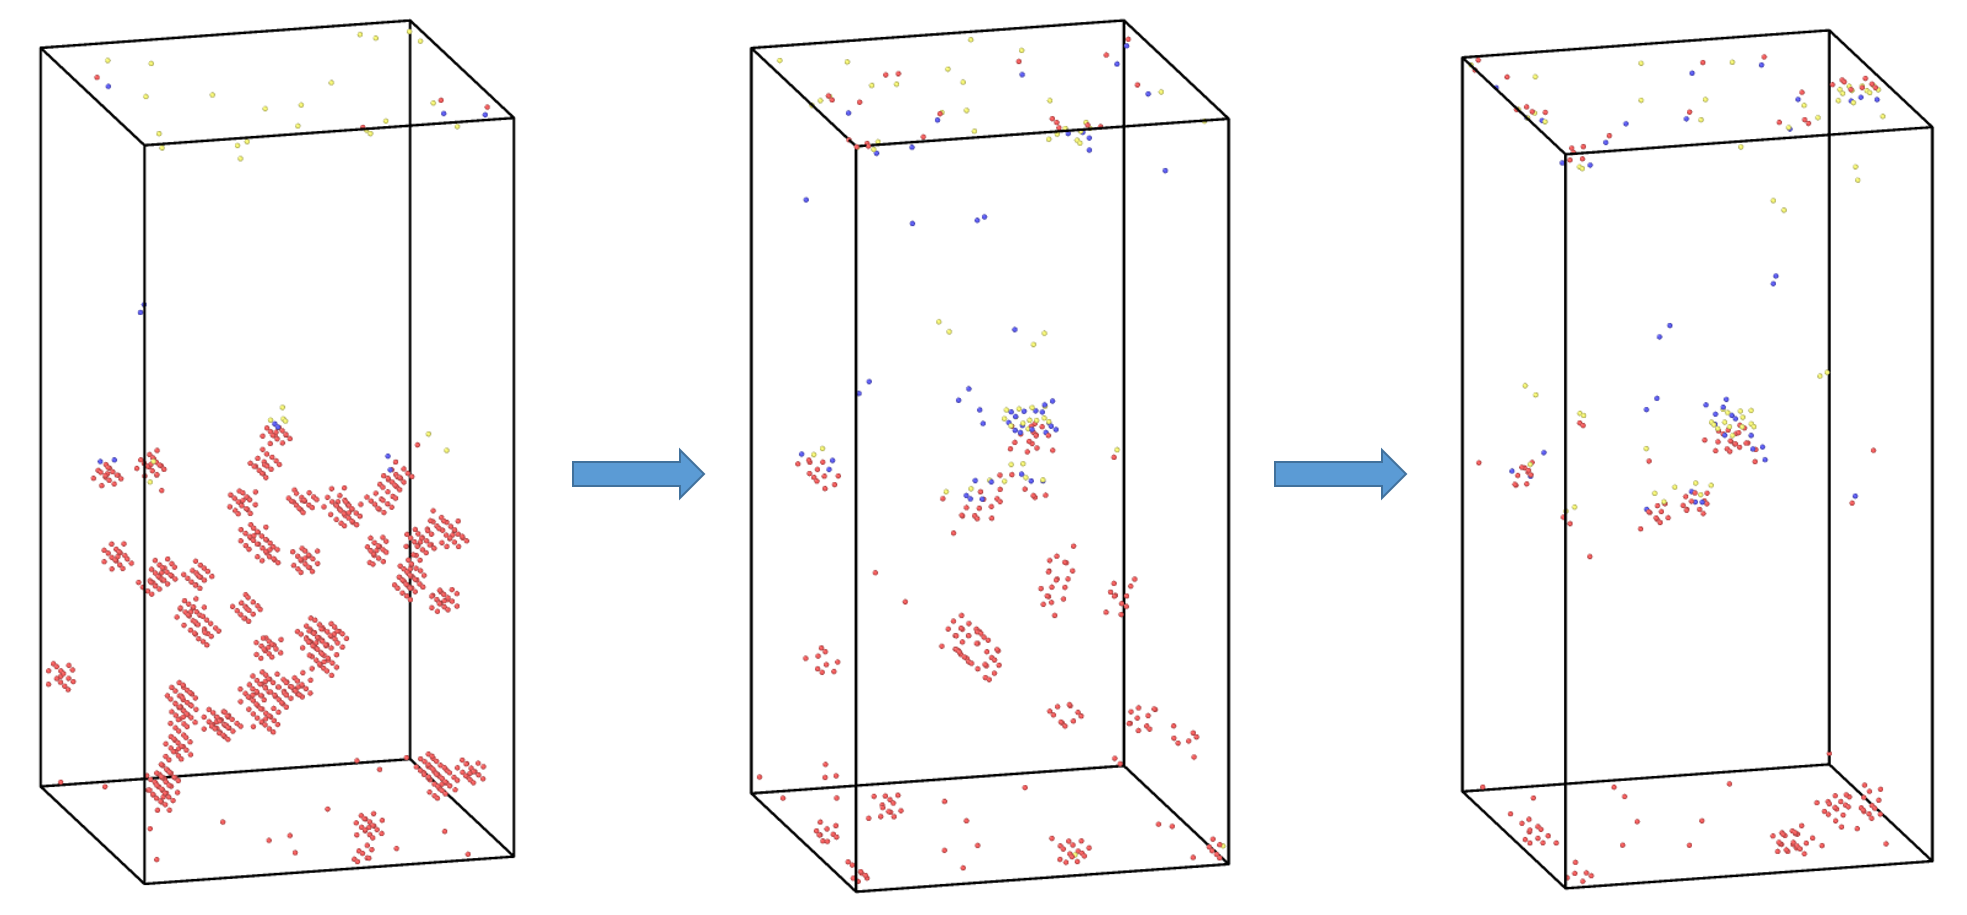
\includegraphics[width=\textwidth]{int_diff_nf.png} 
   \caption{System of BCC-Fe with spherical B2-NiAl precipitate in center of supercell.  Image is a 2-D slice through a 3-D supercell.  Red atoms are Fe; Blue atoms are Ni; Yellow atoms are Al.}
   \label{fig:example}
\end{figure}

\subsubsection{Spherical Precipitates}
Given the high temperature defect behavior results for planar interfaces, it is of interest to determine if similar behavior holds for more realistic spherical precipitates.  In Figure 8, a representative example is displayed of point defects at 600 K near a spherical precipitate.  

It is shown from Figure 8 that similar behavior exists.  Interstitials are diffusing to form clusters and clusters are random walk diffusing throughout the system.  When these clusters find the precipitate, they are pinned on the interface and do not move away from the interface for the remainder of the simulation.  In this system setup, there is much less interfacial area than for planar interfaces in section 4.3.1, and thus the probability of an interstitial cluster diffusing into the precipitate is lower.  Thus, not all of the interstitial clusters have been removed from the bulk.  However, similar behavior is observed in that coherent intermetallic precipitates are functioning to remove point defects from the bulk.

\begin{figure}[htp]
   \centering
   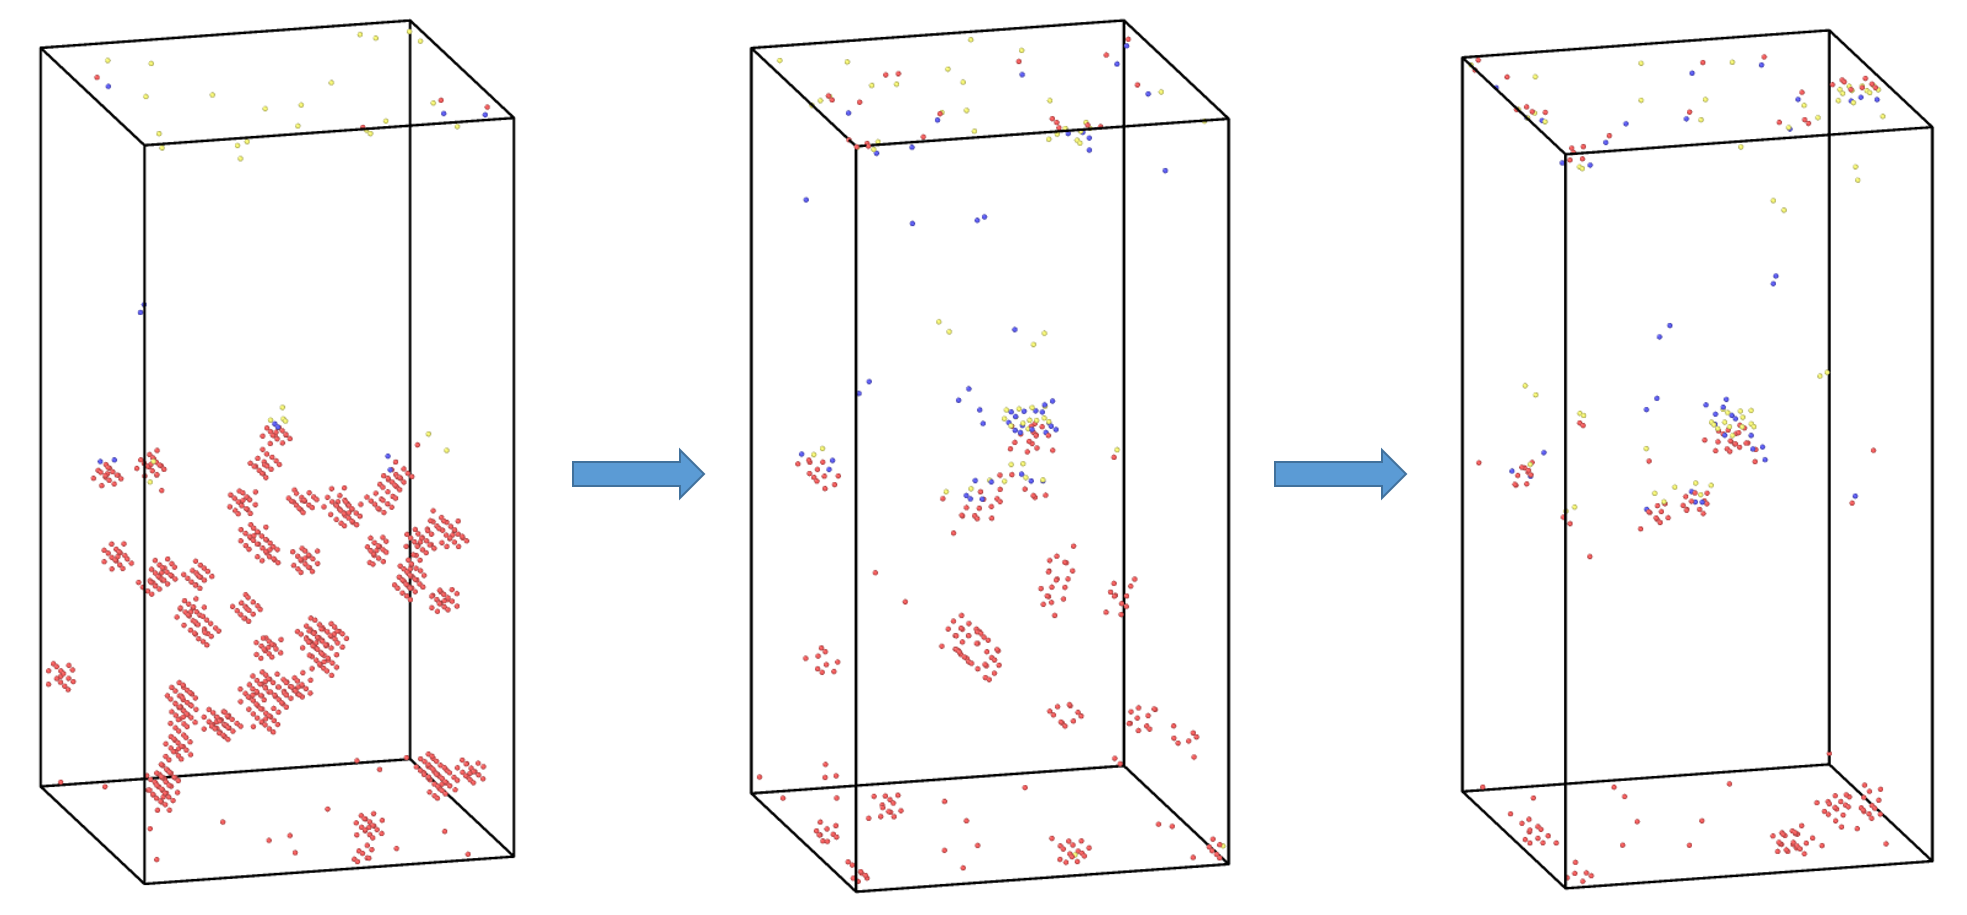
\includegraphics[width=\textwidth]{int_diff_nf.png} 
   \caption{System of BCC-Fe with spherical B2-NiAl precipitate in center of supercell.  Image is a 2-D slice through a 3-D supercell.  Red atoms are Fe; Blue atoms are Ni; Yellow atoms are Al.}
   \label{fig:example}
\end{figure}

\subsection{Radiation Damage Near Interfaces}
\subsubsection{Planar Interfaces}
The final study performed was looking into the effect of interfaces on actual radiation damage behavior.  A two phase system of BCC-Fe and B2-NiAl was generated with a (100) planar interface.  An atom in the Fe matrix was given an additional amount of kinetic energy (5 keV), in a prescribed direction with the primary component towards the interface.  An example cascade is illustrated in Figure 9.  A set of thirty random primary knock-on atom (PKA) directions are utilized in this analysis.  The PKA is progressively moved farther away from the interface, and the effect of the interface on the number of defects produced is analyzed.  A summary of these results is shown in Figure 10.  In Figure 10, the lower dashed line illustrates the number of defects produced in a BCC-Fe system and the upper dashed line illustrates the number of defects produced in a B2-NiAl system from a 5 keV Fe PKA.  It can be seen that when the PKA is very far from the interface, the radiation cascade behaves as if it resided in bulk Fe.  This makes intuitive sense.  As the PKA is moved closer to the interface, the cascade thermal spike begins to interact with the B2-NiAl structure.  It is observed that there exists an increase in the number of defects created from a given PKA as the PKA moves closer to the interface.  This makes sense due to the fact that a higher number of defects are produced from a 5 keV cascade in B2-NiAl than in BCC-Fe.  It should be noted that the interface is stable under irradiation.  However, some substitutional and anti-site defects are formed around the interface region.

\begin{figure}[htp]
   \centering
   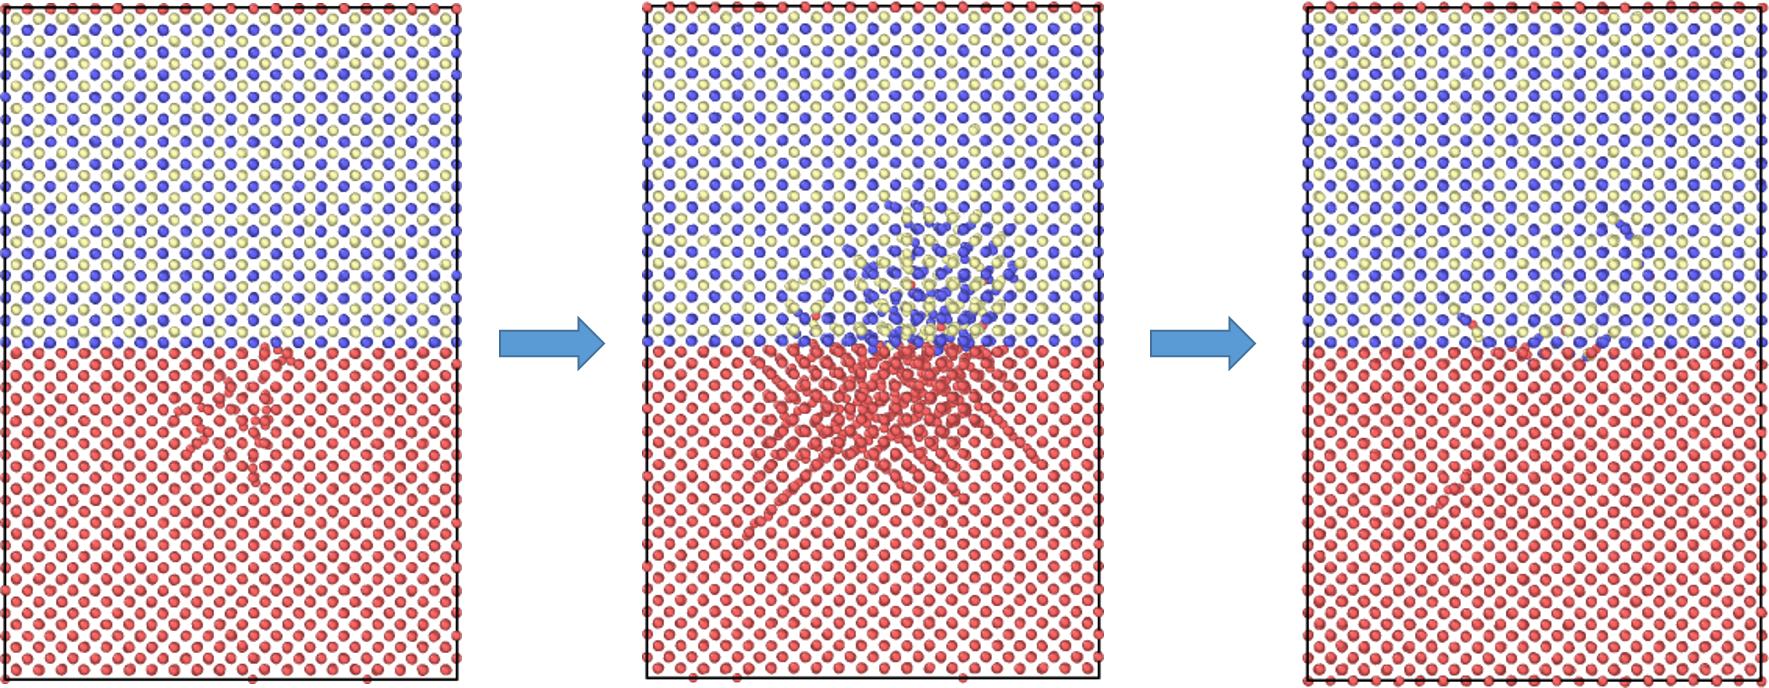
\includegraphics[width=\textwidth]{rad_dam_nf.png} 
   \caption{System of BCC-Fe with spherical B2-NiAl precipitate in center of supercell.  Image is a 2-D slice through a 3-D supercell.  Red atoms are Fe; Blue atoms are Ni; Yellow atoms are Al.}
   \label{fig:example}
\end{figure}

\begin{figure}[htp]
   \centering
   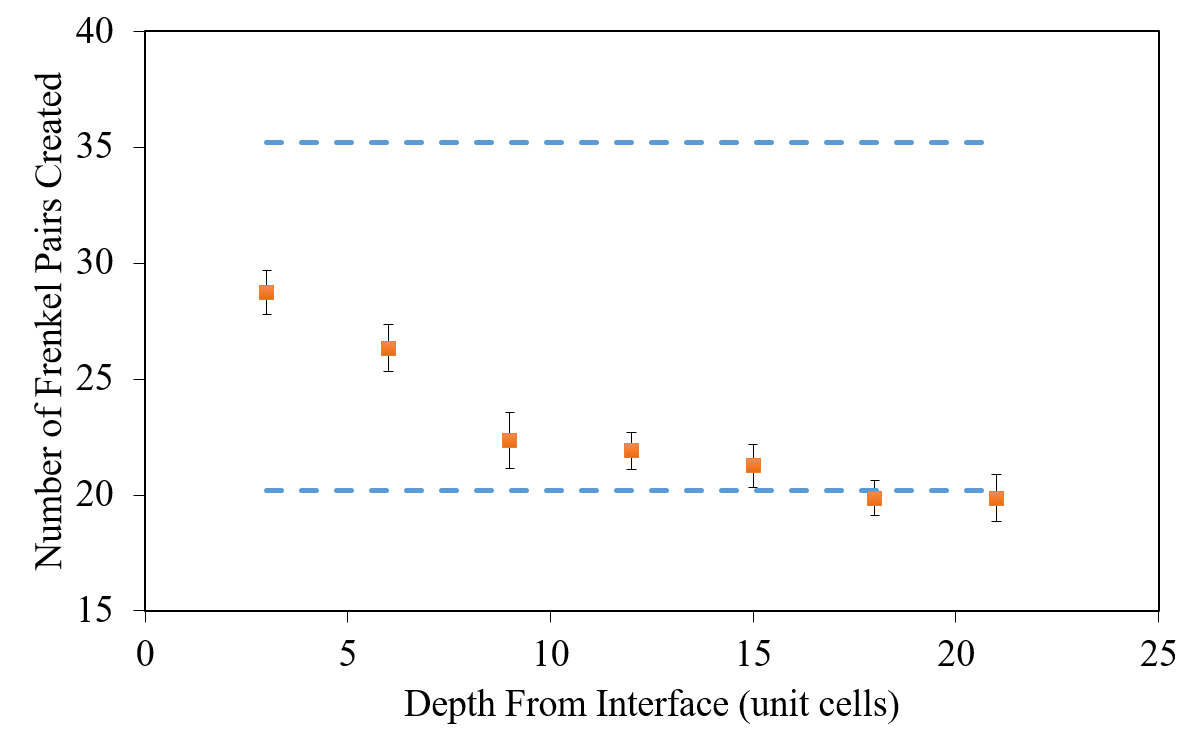
\includegraphics[width=0.5\textwidth]{rad_dam_prof.png} 
   \caption{System of BCC-Fe with spherical B2-NiAl precipitate in center of supercell.  Image is a 2-D slice through a 3-D supercell.  Red atoms are Fe; Blue atoms are Ni; Yellow atoms are Al.}
   \label{fig:example}
\end{figure}

\FloatBarrier
\subsubsection{Spherical Precipitates}
A sphere of B2-NiAl is created within a matrix of BCC-Fe.  As in section 4.4.1, an atom in the Fe matrix was given an additional amount of kinetic energy (5 keV), in a prescribed direction with the primary component towards the precipitate.  An example cascade is illustrated in Figure 11.  


\begin{figure}[htp]
   \centering
   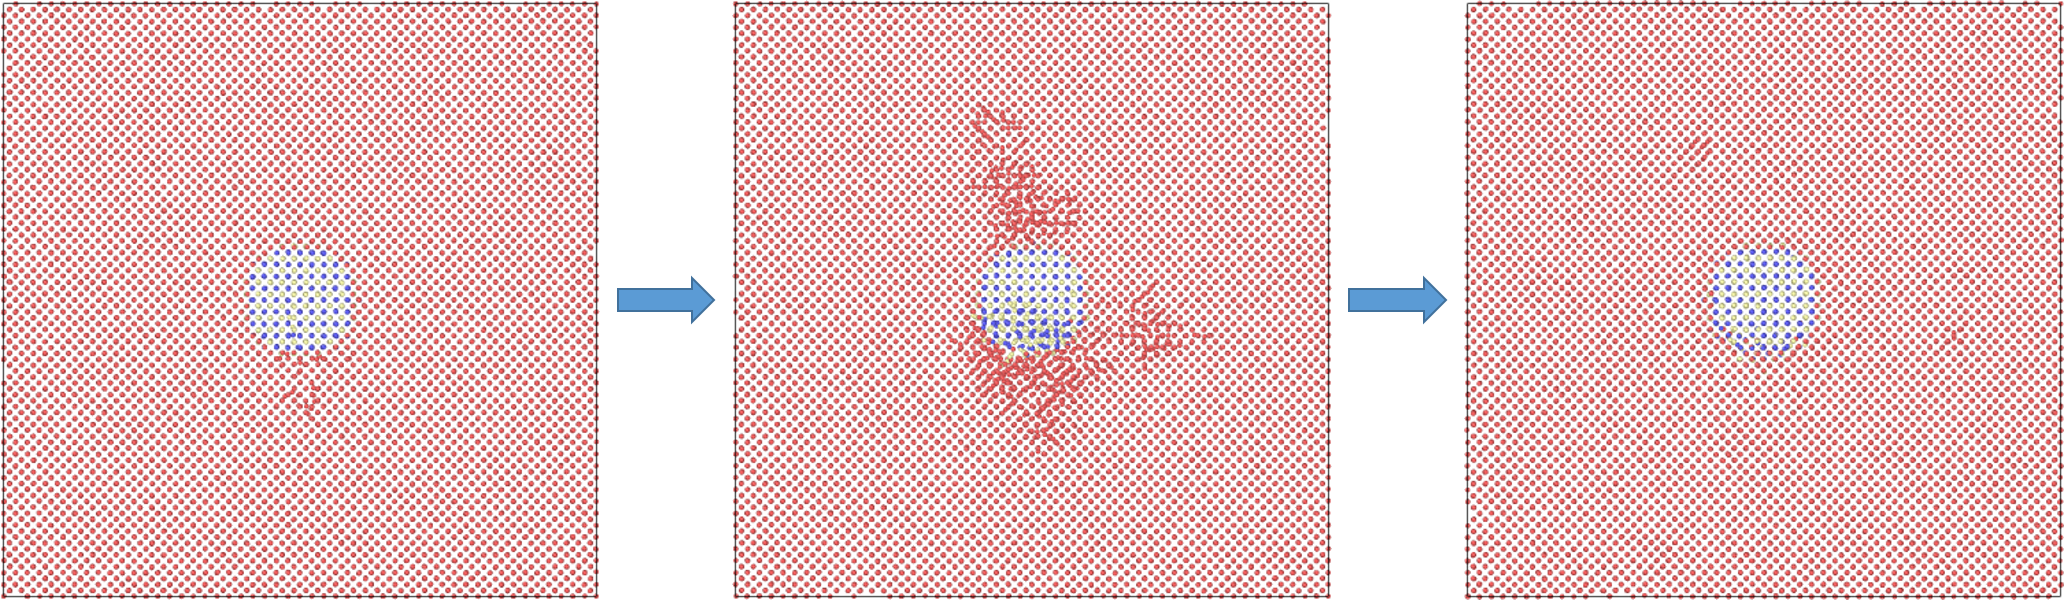
\includegraphics[width=\textwidth]{rad_dam_sphere.png} 
   \caption{System of BCC-Fe with spherical B2-NiAl precipitate in center of supercell.  Image is a 2-D slice through a 3-D supercell.  Red atoms are Fe; Blue atoms are Ni; Yellow atoms are Al.}
   \label{fig:example}
\end{figure}



\FloatBarrier
\section{Conclusions}
This work presented computational investigations aimed at better understanding the role of coherent precipitates in increasing radiation tolerance in maraging steels.  Interatomic potentials were developed for the description of Fe-Ni-Al alloys, to simulate an ideal alloy of BCC Fe with NiAl precipitates, and associated Fe/NiAl planar interfaces.  Characteristics and energetics of the interfaces were analyzed, the interaction of point defects with planar and spherical interfaces was studied, and finally, radiation cascades were induced in proximity to the interfaces.

\section{Acknowledgement}
This work was supported by the US Department of Energy, project $\#$DE-NE0000536000.

\FloatBarrier

\bibliography{bibliography_ben}


\end{document}  
